\def\Ax{0}
\def\Bx{2}
\def\Cx{4}
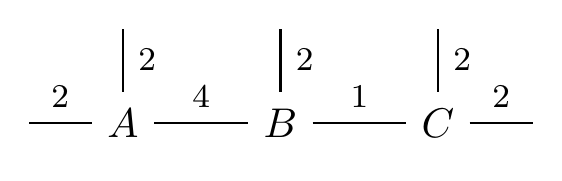
\begin{tikzpicture}[thick, every node/.style={scale=1.5}, tensor/.style={minimum size=0.5cm}]
    \node[tensor] (A) at (\Ax,0) {$A$};
    \node[tensor] (B) at (\Bx,0) {$B$};
    \node[tensor] (C) at (\Cx,0) {$C$};
    
    \draw (A.north) -- +(0,0.8) node[midway, right] {\footnotesize 2};
    \draw (A.west) -- +(-0.8,0) node[midway, above] {\footnotesize 2};
    \draw (B.north) -- +(0,0.8) node[midway, right] {\footnotesize 2};
    \draw (A.east) -- (B.west) node[midway, above] {\footnotesize 4};
    \draw (C.north) -- +(0,0.8) node[midway, right] {\footnotesize 2};
    \draw (C.east) -- +(+0.8,0.0) node[midway, above] {\footnotesize 2};
    \draw (B.east) -- (C.west) node[midway, above] {\footnotesize 1};
\end{tikzpicture}